As análises apresentadas nessa seção resumem os resultados dos apenas executado na extensão feita no Bench4Q. Os resultados aqui mostrados são proporcionados como exemplos de aplicação da metodologia. Dessa forma, para uma melhor abordagem, divide-se os exemplos em  partes:
\begin{itemize}
	\item Configuração da carga no Bench4Q;
	\item Configuração para modular a carga;
	\item Resultado da carga gerada.
\end{itemize}

\begin{figure}[!htb]
	\begin{subfigure}{\linewidth}
		\centering
		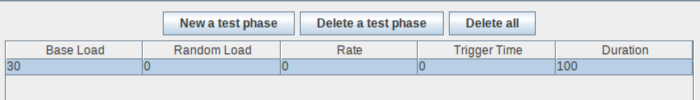
\includegraphics[scale=0.7]{condiguracao-carga-bench4q1.png}
		\caption{Configuração da carga no Bench4Q, para um degrau positivo}
		\label{fig:condiguracao-carga-bench4q1}
	\end{subfigure}\\
	\begin{subfigure}{\linewidth}
		\centering
		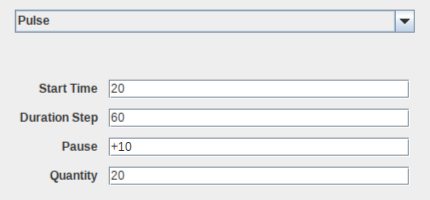
\includegraphics[scale=0.7]{condiguracao-carga-modulada1.png}
		\caption{Configuração para modular a carga como um degrau positivo}
		\label{fig:condiguracao-carga-modulada1}
	\end{subfigure}\\[1ex]
	\begin{subfigure}{\linewidth}
		\centering
		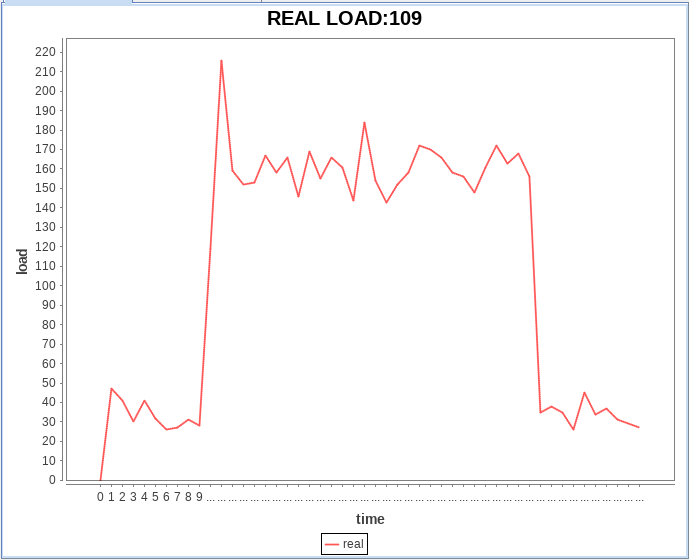
\includegraphics[scale=0.6]{grafico-carga-modulada1.png}
		\caption{Carga gerada com base nas configuração}
		\label{fig:grafico-carga-modulada1}
	\end{subfigure}
	\caption{Carga gerada com base na configuração: Degrau Positivo}
	\label{fig:carga-modulada1}
	\fautor
\end{figure}

A Figura \ref{fig:carga-modulada1} apresenta a primeira exemplificação gerada com o Bench4Q já com a extensão desenvolvida neste trabalho. A figura \ref{fig:condiguracao-carga-bench4q1} demonstra os parâmetros de configuração utilizados para gerar a carga. Dois são os principiais: \textit{Base Load} e \textit{Duration}. O primeiro define a quantidade e EBs envolvidos no experimento, neste caso 30 EBs; já o segundo define o tempo de duração do experimento em segundos, neste caso 100 segundos. Na Figura \ref{fig:condiguracao-carga-modulada1} são apresentados os parâmetros para modular a carga \textit{Start Time} de valor 20, referindo-se ao tempo de espera para o início do restante da carga que se mostra presente e ativa na modulação. Decorrido 20 segundos, 20, dos 30 EBs, definido pelo campo \textit{Quantity} iniciam a geração de carga para o sistema. Essa carga se manterá ativa durante 60 segundos conforme fixado no parâmetro \textit{Duration Step}. Nesse exemplo, o parâmetro \textit{Pause} não apresenta influencia devido ao seu valor 0.
O resultado pode ser analisado através da Figura \ref{fig:grafico-carga-modulada1}. Esse gráfico é nativo do próprio Bench4Q, que demonstra o comportamento da carga no decorrer do tempo. Apesar da estocasticidade a carga, essa modulou-se conforme programado. Essa estocasticidade é característica do Bench4Q, afim de manter reproduzir comportamento realístico como os de clientes acessando um \textit{e-commerce}.

\begin{figure}[!htb]
	\begin{subfigure}{\linewidth}
		\centering
		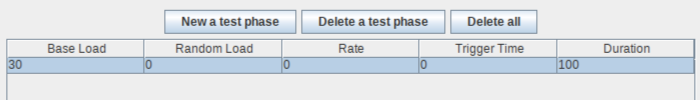
\includegraphics[scale=0.7]{condiguracao-carga-bench4q2.png}
		\caption{Configuração da carga no Bench4Q, para um degrau negativo}
		\label{fig:condiguracao-carga-bench4q2}
	\end{subfigure}\\
	\begin{subfigure}{\linewidth}
		\centering
		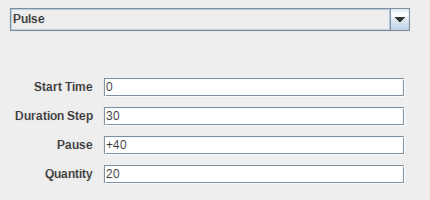
\includegraphics[scale=0.7]{condiguracao-carga-modulada2.png}
		\caption{Configuração para modular a carga como um degrau negativo}
		\label{fig:condiguracao-carga-modulada2}
	\end{subfigure}\\[1ex]
	\begin{subfigure}{\linewidth}
		\centering
		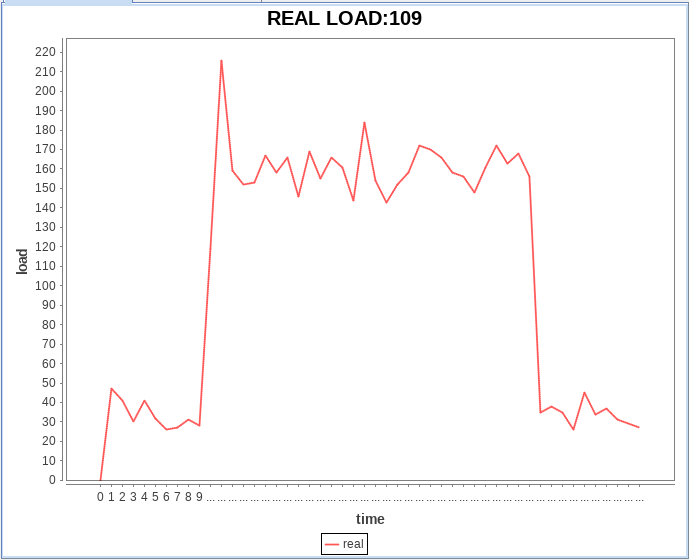
\includegraphics[scale=0.6]{grafico-carga-modulada2.png}
		\caption{Carga gerada com base nas configuração}
		\label{fig:grafico-carga-modulada2}
	\end{subfigure}
	\caption{Carga gerada com base na configuração: Degrau Negativo}
	\label{fig:carga-modulada2}
	\fautor
\end{figure}

A Figura \ref{fig:carga-modulada2} apresenta os resultados dos parâmetros para o objetivo do Degrau Negativo. Os parâmetros de \textit{Base Load} e \textit{Duration} são os mesmos do experimento anterior: 30 EBs e 100 segundos de execução respectivamente, conforme apresentado na Figura \ref{fig:condiguracao-carga-bench4q2}. Já na \ref{fig:condiguracao-carga-modulada3} que demonstra os parâmetros utilizados para modular a carga, o \textit{Start Time} recebe o valor 0, assim a carga modulado iniciar com potência máxima utilizando os 30 EBs sendo 20 EBs setado no \textit{Quantity} para reservá-los para a modulação, o tempo de carga máxima é de 30 segundos como é possível ver no parâmetro \textit{Duration Step}, neste caso o \textit{Pause} é parametrizado com 40 segundos, este valor é o que fará a interrupção brusca dos 20 EBs caindo o nível da geração de carga, gerando o degrau negativo. Passado esse período \textit{Pause}, a carga retorna ao seu nível máximo e atua por mais 30 segundos, o resultado final pode ser visto na Figura \ref{fig:grafico-carga-modulada2}. 
%vale chamar a atenção para a dinâmica apresentada pela geração da carga sempre ao atingir o nivel maximo

\begin{figure}[!htb]
	\begin{subfigure}{\linewidth}
		\centering
		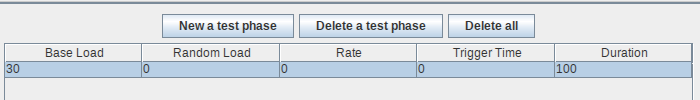
\includegraphics[scale=0.7]{condiguracao-carga-bench4q3.png}
		\caption{Configuração da carga no Bench4Q, para uma onda quadrada}
		\label{fig:condiguracao-carga-bench4q3}
	\end{subfigure}\\
	\begin{subfigure}{\linewidth}
		\centering
		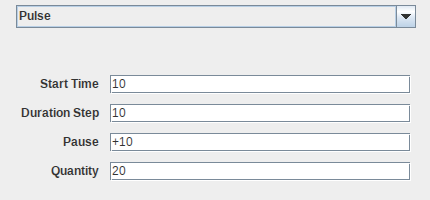
\includegraphics[scale=0.7]{condiguracao-carga-modulada3.png}
		\caption{Configuração para modular a carga como uma onda quadrada}
		\label{fig:condiguracao-carga-modulada3}
	\end{subfigure}\\[1ex]
	\begin{subfigure}{\linewidth}
		\centering
		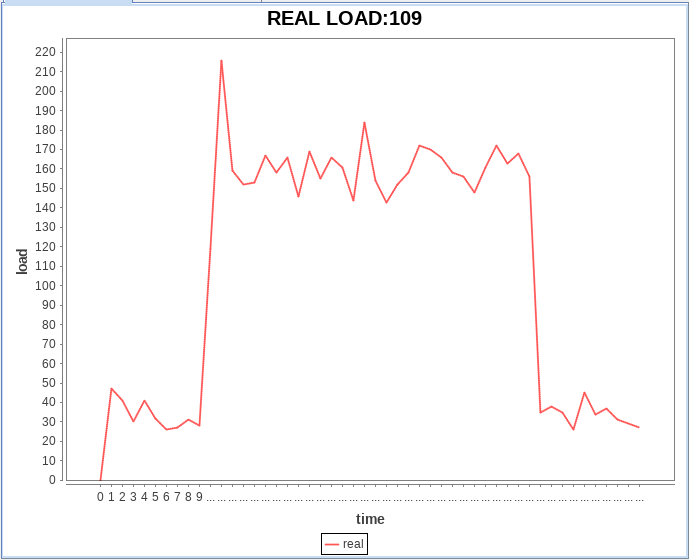
\includegraphics[scale=0.6]{grafico-carga-modulada3.png}
		\caption{Carga gerada com base nas configuração}
		\label{fig:grafico-carga-modulada3}
	\end{subfigure}
	\caption{Carga gerada com base na configuração: Onda Quadrada}
	\label{fig:carga-modulada3}
	\fautor
\end{figure}

A Figura \ref{fig:carga-modulada3} apresenta o resultado da modulação de uma Onda Quadrada. Os parâmetros iniciais do Bench4Q referente a Figura \ref{fig:condiguracao-carga-bench4q3} são os mesmos valores dos outros dois exemplos anteriores. Para gerar uma carga modulada com comportamento oscilatório como a de uma onda quadrada, os parâmetros \ref{fig:condiguracao-carga-modulada3} são definidos com 10 segundos para \textit{Start Time}, 10 segundo de duração para \textit{Duration Step} e 10 para o \textit{Pause}, também configurado com 20 EBs. Para este exemplo vale salientar que para modular a carga como uma onda quadrada dois parâmetros são importantes. \textit{Duration Step} e \textit{Pause}. Esses devem ter os mesmos valores, pois são eles que manterão durante o período definido a carga em níveis baixos e alto. 

\section{Contribuição}
Com a possibilidade da modulação de carga, conforme apresentado na seção anterior, é possível verificar o impacto da carga modulada no ambiente projetado para o trabalho de \citeonline{Edwin2015}. Seguindo o planejamento de experimento apresentado no Capítulo \ref{chapter:metodologia} foi possível coletar dos dados que geram os gráficos a seguir.
Vale lembrar, que foram utilizada dois níveis de cargas de trabalho, 20 e 60 EBs com um unico degrau positivo. Em ambos os casos, foi inicialmente utilizado 40\% da carga até o instante de 30 segundos de experimentação, quando ocorre um crescimento brusco na carga utilizando os 60\% restante da carga, e gerando um degrau positivo. A carga mantém-se máxima, em 100\%, durante 40 segundos (decorridos 70 segundo de experimentação), quando tem uma queda súbita voltando a trabalhar com 40\% da carga até o final do experimento. O objetivo é poder identificar a relação de transformação da entrada na saída, mediante a variação degrau gerada pela carga de trabalho aplicada no sistema.

\begin{figure}[htb]
	\centering
	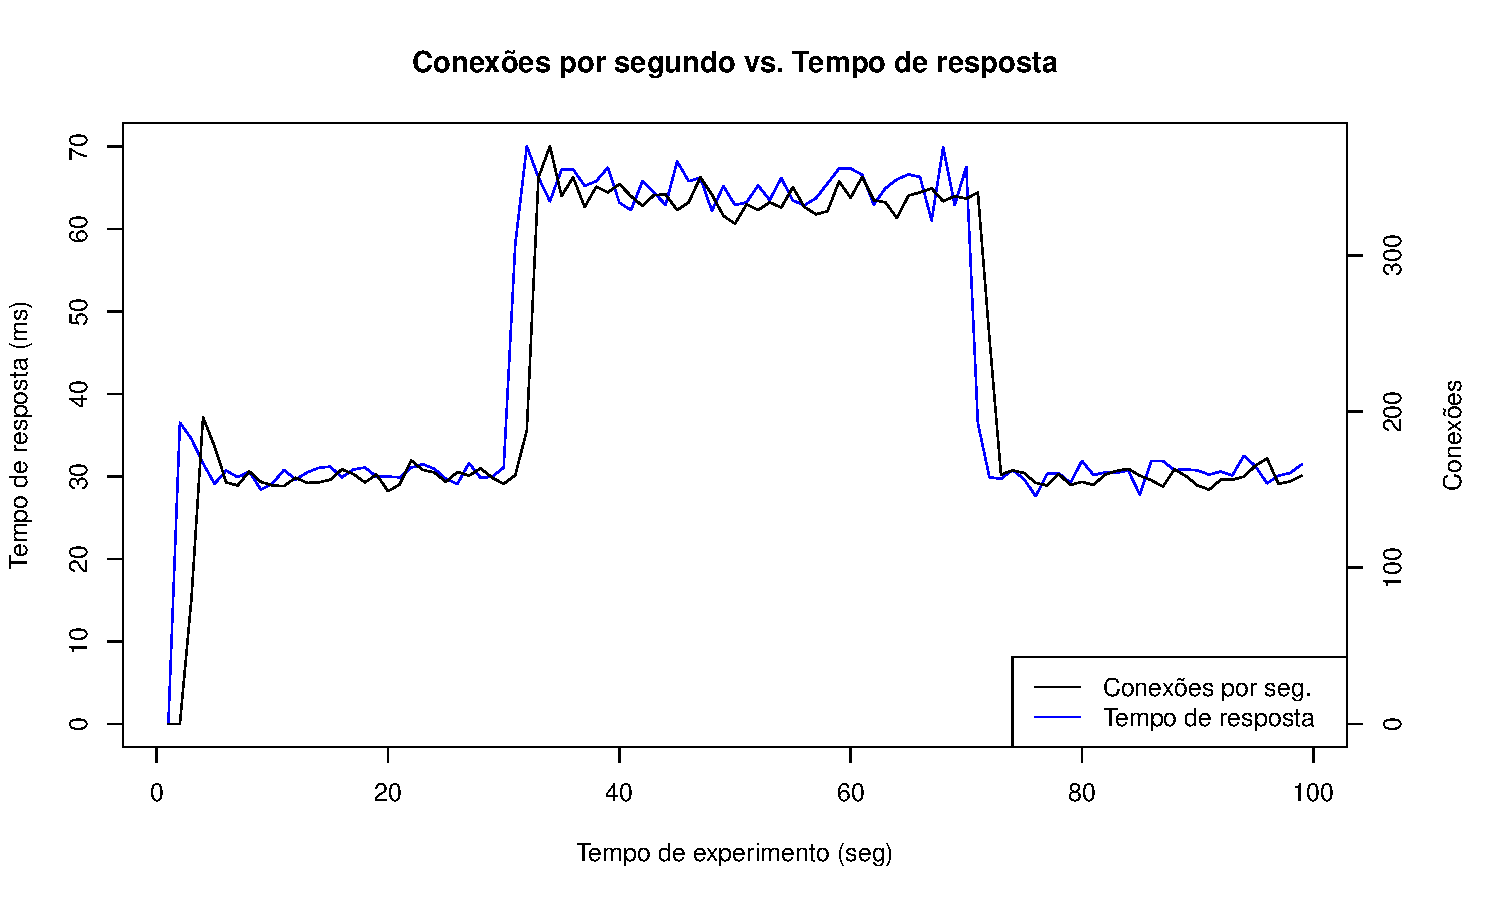
\includegraphics[scale=0.7]{cps-resp60.pdf}	
	\caption{Conexões por segundo vs. Tempo de resposta}
	\label{fig:cps-resp60}
	\fdadospesquisa
\end{figure}

É possível observar a Figura \ref{fig:cps-resp60}, onde são comparados os desempenhos da conexão por segundo e Tempo de resposta. O Bench4Q monitora os tempos de resposta e, no \textit{LoadBalance}, as conexões por segundo. Ao iniciar o experimento é possível verificar a dinâmica da carga em ambas as métricas, seguida por, um assentamento e uma estabilização o instante de 30 segundo de experimentação, neste instante um aumento de carga é aplicado elevando o tempo de resposta e o número de conexões por segundo. Nesse instante é possível verificar novamente a dinâmica do aumento carga no sistema seguido por um assentamento. Essa elevação das métricas se mantem aproximadamente por 70 segundos de experimento quando uma queda acentuada ocorre baixando de desempenho da métrica que se mantem até o final da execução. 
Na Figura \ref{fig:cps-resp60} é possível perceber, em ambas as elevações, que o Tempo de Resposta reage primeiro em comparação ao número de conexões. Isso ocorre devido aos níveis da arquitetura da solução. Esse atraso é referente a dinâmica inerente ao sistema \textit{mult-tiers}. Entretanto, na queda do volume de carga, no intervalo de 70 a 75 segundos, o Tempo de Resposta reage primeiro a queda de carga, quando comparado ao número de conexões por segundo. O tempo de resposta não se apresenta como uma boa métrica de comparação. 

\begin{figure}[htb]
	\centering
	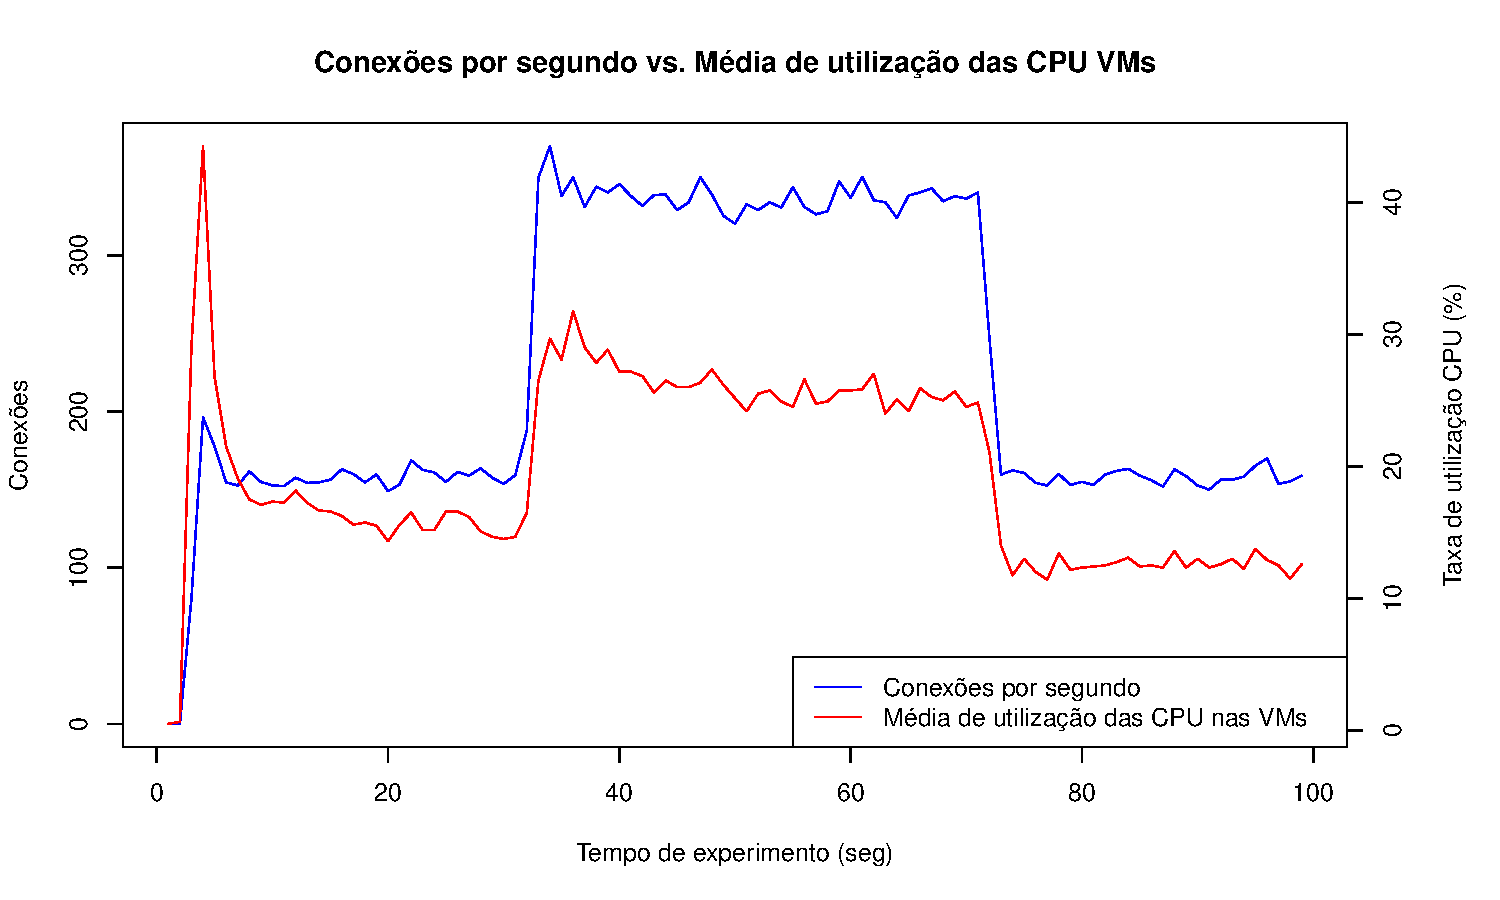
\includegraphics[scale=0.7]{cps-vmcpu60.pdf}
	\caption{Conexões por segundo vs. Média de utilização de CPU nas VMs}
	\label{fig:cps-vmcpu60}
	\fdadospesquisa
\end{figure}

A Figura \ref{fig:cps-vmcpu60} ilustra as conexões por segundos junto com a média da taxa de utilização de CPU nas VMs. No início dos experimentos a utilização de CPU apresenta uma dinâmica acentuada, estacionando em seguida próximo a 13\%. Esse aumento transiente é tão significativo que neste instante chega a atinge a maior média da CPU em todo o experimento, ultrapassando os 40\% de utilização da CPU. Da mesma maneira que o volume de conexões por segundo, a média da taxa de utilização de CPU nas VMs sofre alteração no impacto com o aumento da carga de trabalho próximo aos 30 segundos de experimentação. Decorrido 40 segundos de carga máxima a utilização inicia de maneira mais enfática, atingindo os 30\%. Com o decorrer do período de máximo da carga, a taxa de CPU de maneira tênue a atingir os 23\% aproximadamente. O que chama a atenção na Figura \ref{fig:cps-vmcpu60}, são os trechos de mudança no volume de carga, 0-7, 30-35 e 70-75 segundos aproximadamente. No primeiro instante, de 0 a 7 segundos iniciais, a taxa de utilização sob de maneira busca apresentando uma dinâmica mais acentuada em comparação com o número de conexões por segundo, mesmo que proporcionalmente. Isso é decorrente da inicialização do SUT em cada um dos servidores. A quantidade de tarefas ao iniciar uma aplicação pela primeira vez é maior quando a mesma aplicação é iniciada nas vezes seguinte, devido a inúmeras iterações com outras aplicações para que o serviço fique disponível. Já no intervalo, de 30 a 35 segundos aproximadamente, é possível observar a dinâmica inerente em sistemas multicamadas. O número de conexões por segundo reage a alteração de carga primeiro quando comparada a taxa de utilização sob mesma linha do tempo. Por fim, o trecho de 70 a 75 segundos, o cenário se inverte quando há uma redução na carga de trabalho. A taxa de utilização da CPU reage primeiro a mudança quando comparada com o número de conexões por segundo.

\begin{figure}[htb]
	\centering
	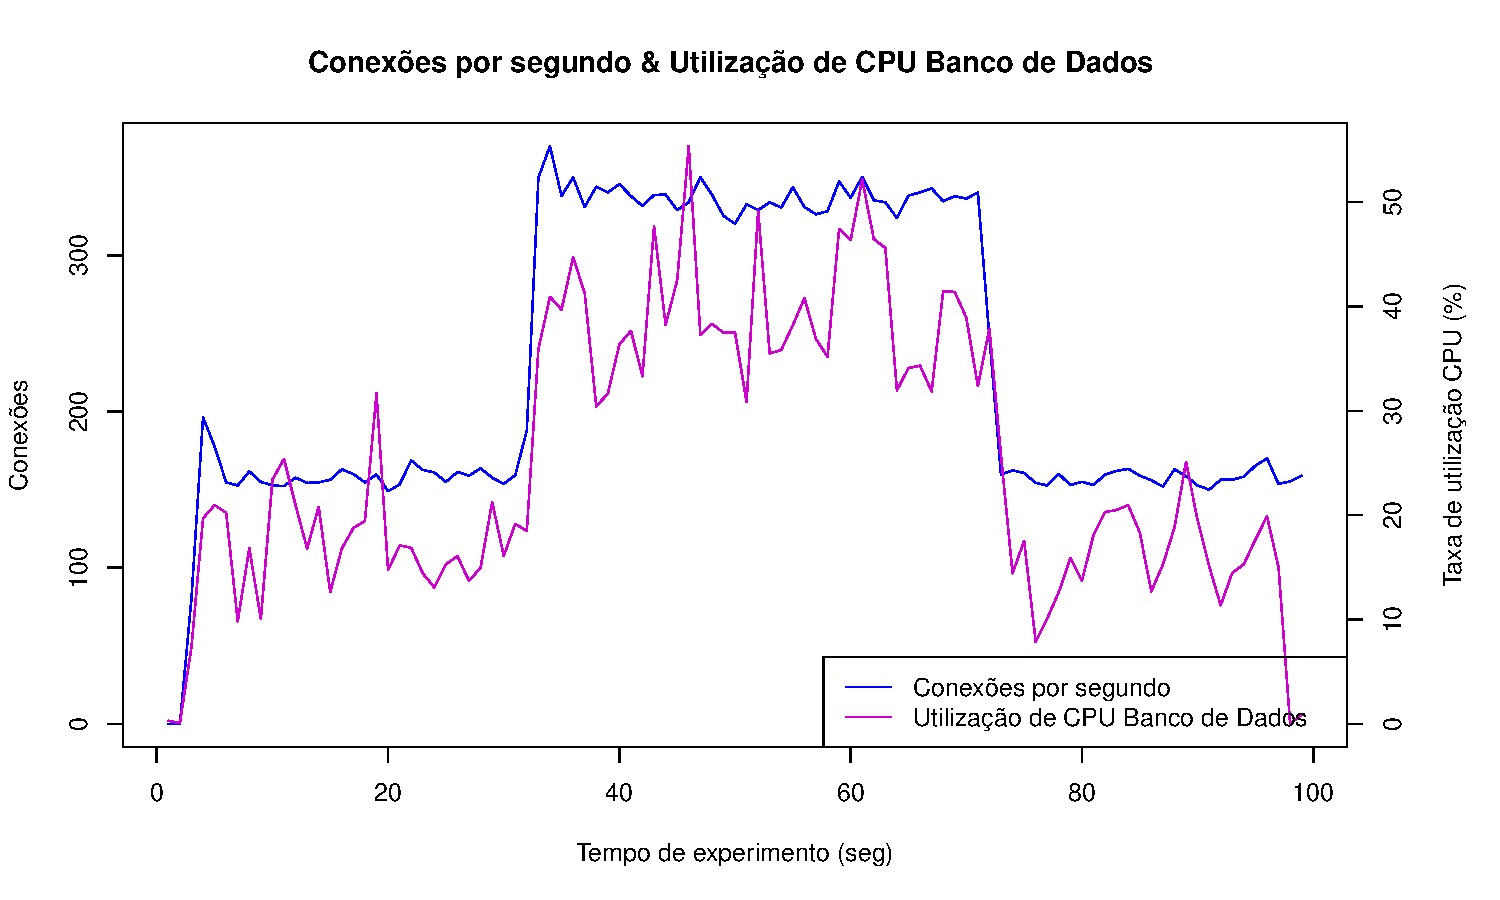
\includegraphics[scale=0.7]{cps-dbcpu60.pdf}
	\caption{Conexões por segundo vs. Utilização de CPU no banco de dados}
	\label{fig:cps-dbcpu60}
	\fdadospesquisa
\end{figure}

Referente a Figura \ref{fig:cps-dbcpu60}, onde se compara o número de conexões por segundo com a Taxa de utilização da CPU no banco de dados, podemos observar uma estocasticidade na taxa de utilização da CPU no banco de dados que está relacionada ao ser o gargalo do sistema. É possível observar a dinâmica de um sistema \textit{multi-tiers}. Do instante 0 até a metade do experimento, o comportamento foi semelhante ao apresentado pela Figura \ref{fig:cps-vmcpu60}, onde o número de conexões por segundo corresponde a taxa de utilização de CPU no banco de dados. Entretanto existe uma convergência no instante da redução da carga de trabalho. Isso se deve ao fato de o banco de dados ter operações em execução mesmo quando foram finalizadas, as consultas por exemplo o encerramento de transações e \textit{commits}. 

\begin{figure}[htb]
	\centering
	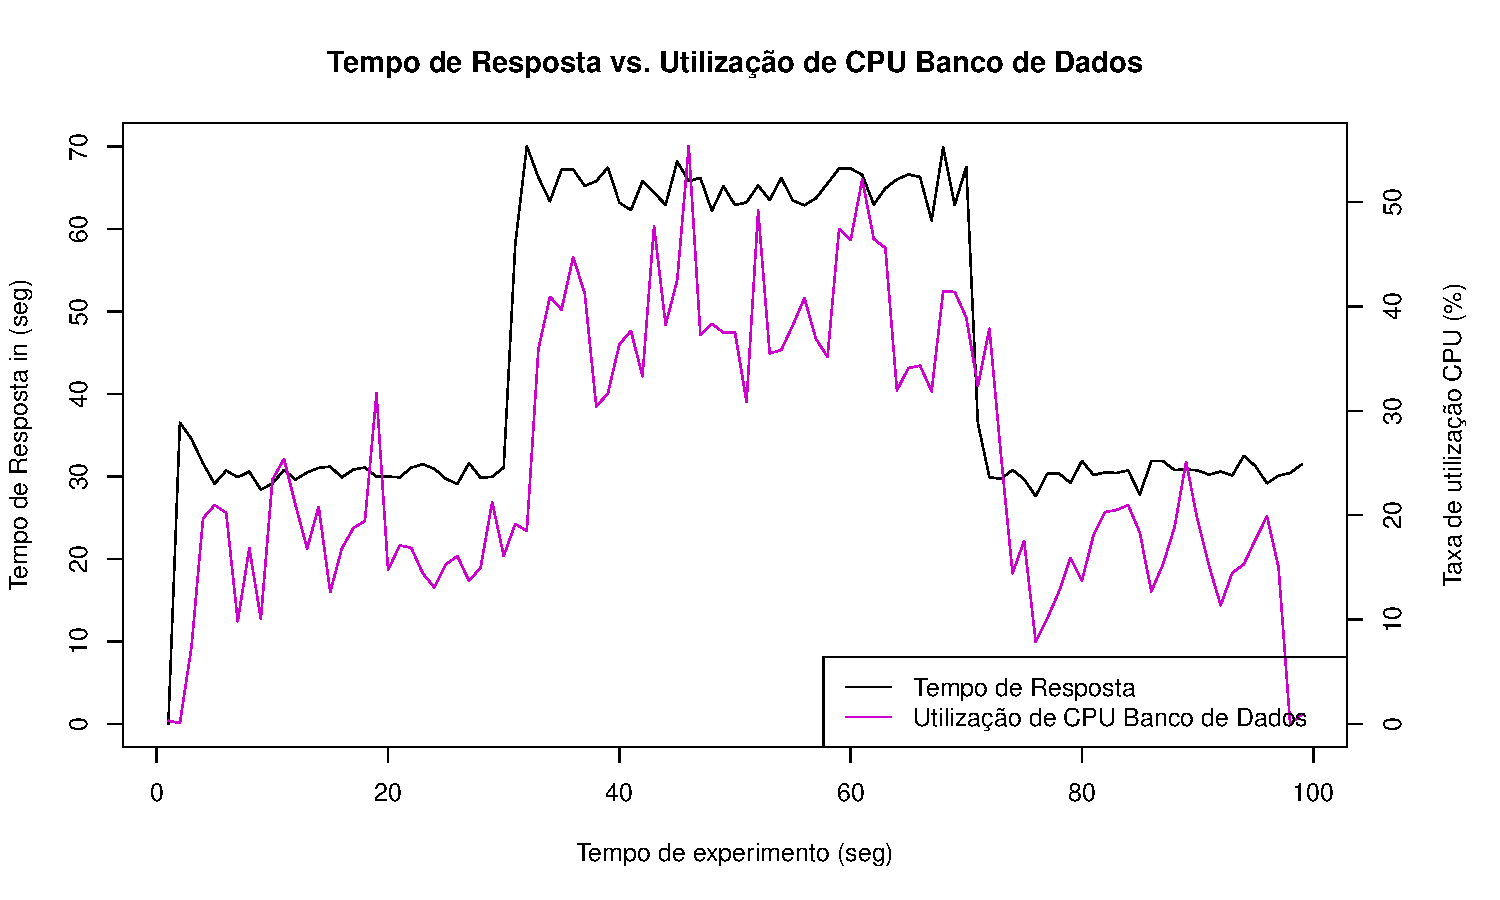
\includegraphics[scale=0.7]{resp-dbcpu60.pdf}
	\caption{Tempo de Resposta vs. Utilização de CPU no banco de dados}
	\label{fig:resp-dbcpu60}
	\fdadospesquisa
\end{figure}

A Figura \ref{fig:resp-dbcpu60} apresenta as duas métricas considerando o ambiente utilizado do experimento. Nela é possível observar novamente a falha gerada pela dinâmica intrínseca quando se lida com sistema \textit{mult-tiers}. O tempo de resposta apresentado é medido no cliente pelo Bench4Q, sendo a camada superior da arquitetura. Já a taxa de utilização da CPU é coletada no banco de dados, estando na camada inferior da arquitetura. Na primeira metade do gráfico, de 0 a 50 segundos, é possível observar o atraso das requisições mediante a transação entre todas as camadas da solução. Já na segunda metade, entre 50 segundos até o final do experimento, podemos observar o atraso novamente, porém este tem um impacto negativo para a métrica de Tempo de Resposta. No trecho de aproximadamente 75 segundos, quando há uma queda na carga de trabalho, o Tempo de Resposta reage primeiro que o consumo de CPU do banco de dados, mascarando o real desempenho da aplicação.
